\documentclass[11pt]{article}
\usepackage[brazilian]{babel}
\usepackage[utf8]{inputenc} %acentuação da língua portuguesa
\usepackage[T1]{fontenc} 
\usepackage{wrapfig} %figura ao lado do texto
\usepackage{graphicx} %pacote de figuras

\usepackage{amsfonts} %pacote com \mathbb{}

\usepackage[pdftex]{hyperref} %links da internet

\usepackage{fancyhdr} 

\usepackage{hyphenat} %retirar hefenação

\tolerance=1 %retirar hefenação

\emergencystretch=\maxdimen %retirar hefenação

\hyphenpenalty=10000 %retirar hefenação

\hbadness=10000 %retirar hefenação

\hyphenchar\font=-1 %retirar hefenação

\sloppy %retirar hefenação

\usepackage{textcomp}

\usepackage[a4paper,left=2cm,right=2cm,top=2.5cm,bottom=2cm]{geometry}

\setlength{\parindent}{0pt} %Parágrafo sem identação]

\begin{document}
	
\pagestyle{fancy}
\renewcommand{\headrulewidth}{0pt}
\renewcommand{\footrulewidth}{2.1pt}
\fancyfoot[L]{\small Diego Silveira Costa Nascimento}
\fancyfoot[R]{\small diego.nascimento@ifrn.edu.br}
	
\begin{minipage}[c][1.5cm][c]{3cm}
	\begin{flushleft}
		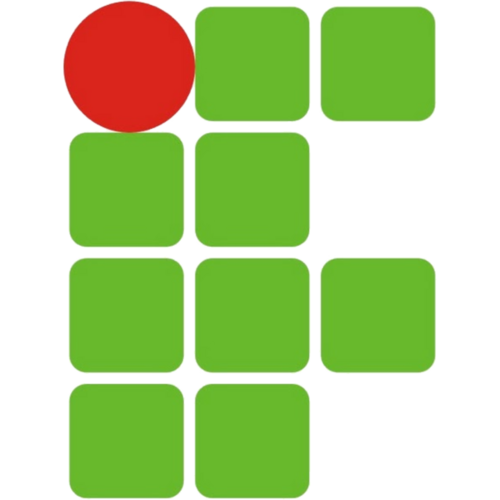
\includegraphics[scale=0.25]{IFRN}
	\end{flushleft}
\end{minipage}		
\begin{minipage}[c][1.5cm][c]{10.8cm}
	\begin{center}
		\resizebox{!}{0.3cm}{\textbf{Fundamentos de Programação}}\par
		\resizebox{!}{0.2cm}{\textbf{Instituto Federal de Educação, Ciência e Tecnologia do Rio Grande do Norte}}\par
		\resizebox{!}{0.2cm}{\today}
	\end{center}
\end{minipage}

\begin{center}
Exercícios
\end{center}

\section{Instrução de Saída}

\begin{enumerate}

\item Implementar um programa que exiba na tela a mensagem: Oi, seu nome!.

\item Implementar um programa que exiba na tela os nomes dos meses do ano separadas por quebra
de linha.

\item Implementar um programa que exiba na tela os nomes dos meses do ano separados por vírgula
em uma única linha.

\item  Implementar um programa que exiba na tela as letras do alfabeto separadas por quebra de linha.

\item Implementar um programa que exiba na tela as letras do alfabeto separados por vírgula em uma
única linha.

\item  Implementar um programa que exiba na tela as letras do alfabeto em grupo de 3 letras separados
por quebra de linha.

\item Implementar um programa que exiba na tela um quadrado formado por caracteres *.

\item Implementar um programa que exiba na tela um triângulo formado pelos caracteres /,\textbackslash
e \_.

\item  Implementar um programa que exiba na tela as letras IF usando símbolos.

\item  Implementar um programa que exiba na tela o calendário do mês corrente.

\end{enumerate}

\newpage

\section{Instrução de Entrada}

\begin{enumerate}
	
	\item Implementar um programa que leia um valor literal via teclado, e como saída, exiba na tela a
	mensagem ``Oi, nome da pessoa!''.
	
	\item Implementar um programa que leia dois valores literais via teclado, correspondentes ao nome e
	sobrenome, e como saída, exiba na tela o nome completo em uma única linha.
	
	\item  Implementar um programa que leia cinco valores literais via teclado, correspondentes as vogais
	do alfabeto, e como saída, exiba na tela cada letra separadas por quebra de linha.
	
	\item  Implementar um programa que leia cinco valores literais via teclado, correspondentes as vogais
	do alfabeto, e como saída, exiba na tela cada letra separadas por vírgulas em uma única linha.
	
	\item Implementar um programa que leia 26 valores literais via teclado, correspondentes as letras do
	alfabeto, e como saída, exiba na tela cada letra separadas por quebra de linha.
	
	\item Implementar um programa que leia 26 valores literais via teclado, correspondentes as letras do
	alfabeto, e como saída, exiba na tela cada letra separadas por vírgulas em uma única linha.
	
	\item Implementar um programa que leia um valor literal via teclado, correspondente ao nome de uma
	fruta, e como saída, exiba na tela a mensagem conforme formato a seguir:
	
	-- -- --\\
	Fruta\\
	-- -- --
	
	\item Implementar um programa que leia um valor literal e três valores inteiros via teclado,
	correspondentes ao nome, dia, mês e ano de nascimento, e como saída, exiba na tela a mensagem
	conforme formato a seguir:
	
	-- -- -- -- -- -- -- -- -- -- -- -- -- -- -- -- -- -- --\\
	Nome: nome\\
	Data de nascimento: dia/mês/ano\\
	-- -- -- -- -- -- -- -- -- -- -- -- -- -- -- -- -- -- --
\end{enumerate}

\newpage

\section{Operadores Aritméticos e Atribuição}

\begin{enumerate}
	\item Implementar um programa que leia dois valores reais via teclado, em seguida, calcule a soma
	entre eles, e como saída, exiba na tela o resultado.
	
	\item  Implementar um programa que leia dois valores reais via teclado, em seguida, calcule a subtração
	entre eles, e como saída, exiba na tela o resultado.
	
	\item Implementar um programa que leia dois valores reais via teclado, em seguida, calcule a
	multiplicação entre eles, e como saída, exiba na tela o resultado.
	
	\item  Implementar um programa que leia dois valores reais via teclado, em seguida, calcule a divisão
	entre eles, e como saída, exiba na tela o resultado.
	
	\item Implementar um programa que leia dois valores inteiros via teclado, em seguida, calcule a divisão
	entre eles, e como saída, exiba na tela o dividendo, o divisor, o quociente e o resto.
	
	\item Implementar um programa que leia um valor real positivo ou negativo via teclado, em seguida
	calcule o valor simétrico $s$ (de acordo com a fórmula: $s = n \times -1)$, e como saída, exiba na tela o
	resultado.
	
	\item Implementar um programa que leia um valor real via teclado, correspondente ao radicando $n$ de
	uma raiz $r$, em seguida, calcule a raiz quadrada (de acordo com a fórmula: $r = n^{\frac{1}{2}}$), e como
	saída, exiba na tela o resultado.
	
	\item  Implementar um programa que leia dois números reais via teclado, correspondentes ao radicando
	$n$ e a ordem $x$ de uma raiz $r$, em seguida calcule a raiz de qualquer ordem (de acordo com a
	fórmula: $r = n^{\frac{1}{x}}$), e como saída, exiba na tela o resultado.
	
	\item Implementar um programa que leia três valores reais via teclado, correspondentes as notas de um
	aluno, em seguida, calcule a média aritmética entre elas, e como saída, exiba na tela o resultado.
	
	\item Implementar um programa que leia três valores reais via teclado, correspondente as notas de
	um aluno, em seguida, calcule a média ponderada entre elas (assumir os valores 3, 3 e 4 para os
	pesos das notas), e como saída, exiba na tela o resultado.
	
	\item  Implementar um programa que leia um valor inteiro via teclado, em seguida, construa as tabuadas
	de 1 a 10 para as operações aritméticas de soma e multiplicação, e como saída, exiba na tela
	todos os resultados.
	
	\item Implementar um programa que leia um valor real via teclado, correspondente a temperatura em
	graus Celsius $^{\circ}C$, em seguida calcule a conversão para graus Fahrenheit $^{\circ}F$ (de acordo com a fórmula:
	$^{\circ}F = ^{\circ}C \times 1.8 + 32$), e como saída, exiba na tela o resultado.
	
	\item Implementar um programa que leia um valor real via teclado, correspondente à base $b$ do
	quadrado, em seguida, calcule a área $a$ (de acordo com a fórmula: $a = b^{2}$, e como saída, exiba o
	resultado na tela.
	
	\item Implementar um programa que leia dois valores reais via teclado, correspondentes a base $b$ e
	altura $h$ de um retângulo, em seguida calcule a área $a$ (de acordo com a fórmula: $a = b \times h$), e
	como saída, exiba na tela o resultado.
	
	\item  Implementar um programa que leia dois valores reais via teclado, correspondentes a base $b$ e
	altura $h$ de um triângulo, calcule a área $a$ (de acordo com a fórmula: $a = \frac{b \times h}{2}$), e como saída,
	exiba o resultado na tela.
	
	\item  Implementar um programa que leia um valor real via teclado, correspondente ao raio $r$ de um
	círculo, em seguida, calcule a área $a$ (de acordo com a fórmula: $a = 3.14 \times r^{2}$), e como saída,
	exiba na tela o resultado.
	
	\item Implementar um programa que leia dois valores reais via teclado, correspondentes aos valores dos
	catetos $a$ e $b$ de um triângulo retângulo, em seguida, calcule o valor da hipotenusa $h$ (de acordo
	com a fórmula: $h = \sqrt{a^{2} + b^{2}}$), e como saída, exiba na tela o resultado.
	
	\item Implementar um programa que leia dois valores reais via teclado, correspondente ao valor de um
	produto e o seu desconto, em seguida, calcule o valor a ser pago pelo produto, e como saída,
	exiba na tela o resultado.
	
	\item Implementar um programa que leia três valores reais via teclado, correspondente ao valor de um
	produto, a quantidade e o seu desconto, em seguida, calcule o valor a ser pago pelo produto, e
	como saída, exiba na tela o resultado.
	
	\item  Implementar um programa que leia cinco valores inteiros via teclado, correspondente a quantidade
	de votos de cada candidato, em seguida, calcule a porcentagem dos votos, e como saída, exiba
	na tela o resultado da eleição.
	
	\item  Implementar um programa que leia um valor inteiro via teclado, correspondente a altura $a$ de
	um homem, em seguida, calcule o peso ideal $p$ (de acordo com a fórmula: $p = (72.7 \times a) - 58$),
	e como saída, exiba na tela o resultado.
	
	\item Implementar um programa que leia um valor inteiro vai teclado, correspondente a altura $a$ de
	uma mulher, em seguida, calcule o peso ideal $p$ (de acordo com a fórmula: $p = (62.1 \times a) - 44.7$),
	e como saída, exiba na tela o resultado.
	
	\item  Implementar um programa que leia dois valores inteiros em variáveis separadas, por exemplo,
	``valor1'' e ``valor2'', e em seguida, troque os valores entre elas usando uma variável auxiliar, e
	como saída, exiba na tela os valores atualizados para ``valor1'' e ``valor2''.
	
	\item Implementar um programa que leia um valor inteiro de quatro dígitos via teclado, em seguida,
	desmembre-o em unidade, dezena, centena e milhar, e como saída, exiba na tela os valores de
	unidade, dezena, centena e milhar.
	
	\item  Implementar um programa que leia um valor inteiro de quatro dígitos via teclado, em seguida,
	inverta os valores de trás para frente formando um único número, e como saída, exiba na tela o
	novo número.
\end{enumerate}

\newpage

\section{Estrutura de Seleção}

\begin{enumerate}
	\item Implementar um programa que leia um valor inteiro via teclado, em seguida verifique se o número
	é positivo ou negativo, e como saída, exiba na tela a mensagem ``O número é positivo'' ou ``O
	número é negativo''.
	
	\item  Implementar um programa que leia um valor real via teclado, que corresponde à temperatura de
	de um paciente, em seguida, verifique se o paciente apresenta febre ou não (tomar como base a
	temperatura maior que 36.5 $^{\circ}C$ para febre), e como saída, exiba na tela a mensagem ``Paciente
	apresenta febre'' ou ``Paciente não apresenta febre''.
	
	\item  Implementar um programa que leia um valor inteiro entre 1 e 12 via teclado, em seguida, compare
	ao valor de mês do ano, e como saída, exiba na tela o nome do mês do ano correspondente, ou a
	mensagem ``Mês do ano inválido!''.
	
	\item Implementar um Programa que leia valor inteiro via teclado, em seguida, compare ao valor do
	dia da semana, e como saída, exiba na tela o nome do dia da semana, ou a mensagem ``Dia da
	semana inválido''.
	
	\item  Implementar um programa que leia dois valores reais vai teclado, que correspondem as notas de
	aluno, em seguida, calcule a sua média, e como saída exiba na tela o conceito da média (Entre
	9.0 e 10.0 – conceito A; entre 7.5 e 9.0 – conceito B; entre 6.0 e 7.5 – conceito - C; entre 4.0 e
	6.0 – conceito D; e entre 4.0 e zero – conceito E).
	
	\item  Implementar um programa que leia dois valores inteiros via teclado, em seguida, verifique se os
	valores são iguais, e como saída, exiba na tela a mensagem ``Os valores são iguais'' ou ``Os valores
	são diferentes''.
	
	\item Implementar um programa que leia dois valores reais via teclado, em seguida, verifique qual é o
	menor, e como saída, exiba na tela o menor valor.
	
	\item Implementar um programa que leia dois valores reais via teclado, em seguida, verifique qual é o
	maior, e como saída, exiba na tela o maior valor.
	
	\item Implementar um programa que leia um valor inteiro via teclado, em seguida verifique se o número
	é par ou ímpar (um número é par quando o resto da divisão por dois é igual a zero), e como
	saída, exiba na tela a mensagem ``O número é par'' ou ``O número é ímpar''.
	
	\item Implementar um programa que leia dois valores reais via teclado, que correspondem as notas de
	um aluno, em seguida, calcule a média aritmética entre elas e verifique se o aluno está aprovado
	ou reprovado (o aluno é aprovado quando a média for maior ou igual a 7), e como saída, exiba
	na tela a mensagem ``Aluno aprovado'' ou ``Aluno reprovado''.
	
	\item Implementar um programa que leia um valor literal via teclado, em seguida, verifique se é uma
	vogal ou consoante, e como saída, exiba na tela a mensagem ``A letra é uma vogal'' ou ``A letra é
	uma consoante''.
	
	\item Implementar um programa que leita um valor inteiro via teclado, que corresponde a um ano do
	calendário gregoriano, em seguida, verificar se o ano é bissexto ou não (o ano é bissexto quando
	é múltiplo de 400, ou quando é múltiplo de 4 e não é múltiplo de 100), e como saída, exiba na
	tela a mensagem ``O ano é bissexto'' ou ``O ano não é bissexto''.
	
	\item  Implementar um programa que leia três valores reais via teclado, que correspondem aos
	coeficientes $a$, $b$ e $c$ de uma equação de segundo grau $ax^{2} + bx + c$, em seguida, calcule o valor
	de delta $d$ (de acordo com a fórmula: $d = b^{2} - 4 \times a \times c$) e as raízes de uma equação do segundo
	grau $x'$ e $x''$ (sendo $x'= \frac{-b + \sqrt{d}}{2 \times a}$ e $x''= \frac{-b - \sqrt{d}}{2 \times a}$), e como saída, exiba na tela os valores de $x'$
	e $x''$, ou a mensagem ``A equação não tem raízes'', caso do valor de delta ser negativo.
	
	\item Implementar um programa que leia dois valores reais e um valor literal ($+$, $-$ , $\times$ e $/$) via teclado,
	em seguida, calcule a operação aritmética de acordo com a opção digitada, e como saída, exiba
	na tela o resultado.
	
	\item Implementar um programa que leia três valores diferentes reais via teclado, em seguida, faça uma
	comparação entre eles, e como saída, exiba na tela o menor valor.
	
	\item  Implementar um programa que leia três valores diferentes reais via teclado, em seguida, faça uma
	comparação entre eles, e como saída, exiba na tela o maior valor.
	
	\item Implementar um programa que leia três valores diferentes reais via teclado, em seguida, faça uma
	comparação entre eles, e como saída, exiba na tela o valor intermediário
	
	\item As Organizações Tabajara resolveram dar um aumento de salário aos seus colaboradores e lhe
	contrataram para construir um programa que calculará os reajustes. Implemente um programa
	que leia um valor real via teclado, que corresponde ao salário de um colaborador, em seguida,
	calcule o reajuste segundo os critério baseado no salário atual (Salários até R\$ 280,00 - aumento
	de 20\%; salários entre R\$ 280,00 e R\$ 700,00 - aumento de 15\%; salários entre R\$ 700,00 e R\$
	1.500,00 - aumento de 10\%; e salários de R\$ 1.500,00 em diante - aumento de 5\%.), e como saída,
	exiba na tela o salário antes do reajuste, o percentual de aumento aplicado, o valor do aumento
	e o novo salário, após o aumento.
\end{enumerate}

\newpage

\section{Estrutura de Repetição: while}

\begin{enumerate}
	\item  Implementar um programa que exiba na tela uma contagem de 1 até 1000.
	
	\item Implementar um programa que exiba na tela os números pares de uma contagem de 1 até 1000.
	
	\item Implementar um programa que exiba na tela os números ímpares de uma contagem de 1 até
	1000.
	
	\item Implementar um programa que leia 10 valores inteiros via teclado, e como saída, exiba na tela o
	resultado da soma.
	
	\item Implementar um programa que leia 20 valores reais via teclado, e como saída, exiba na tela o
	resultado da média.
	
	\item Implementar um programa que leia 15 valores inteiros via teclado, e como saída, exiba na tela o
	menor valor.
	
	\item  Implementar um programa que leia 15 valores inteiros via teclado, e como saída, exiba na tela o
	maior valor.
	
	\item Implementar um programa que leia 10 valores reais via teclado, e como saída, exiba o menor
	valor, o maior valor e a média de todos os valores.
	
	\item Implementar um programa que leia um valor inteiro via teclado, em seguida, calcule o fatorial de
	um número (O fatorial de $5! = 5 \times 4 \times 3 \times 2 \times 1 = 120$), e como saída, exiba na tela o resultado.
	
	\item  Implementar um programa que leia um valor inteiro via teclado, que corresponde o número de
	termos de uma série de Fibonacci (1, 1, 2, 3, 5, 8, 13, 21, 34, 55, ...), e como saída, exiba na tela
	cada valor da sequência.
	
	\item  Implementar um programa que leia um valor inteiro via teclado, e como saída, exibir na tela se
	o valor é primo ou não (O número é primo quando é divisível por um e por ele mesmo).
	
	\item  Implementar um programa que leia dois valores inteiros via teclado, sendo o primeiro menor que
	o segundo, e como saída, exibir apenas os números primos do início ao fim da sequência.
	
	\item Supondo que a população de um país A seja da ordem de 80.000 habitantes com uma taxa
	anual de crescimento de 3\% e que a população de B seja 200.000 habitantes com uma taxa de
	crescimento de 1.5\%. Implemente um programa que exiba na tela o valor de crescimento de cada
	país ao ano até que país A ultrapasse ou iguale a população do país B.
\end{enumerate}

\newpage

\section{Estrutura de Repetição: for}

\begin{enumerate}
	\item  Implementar um programa que exiba na tela uma contagem de 1 até 1000.
	
	\item Implementar um programa que exiba na tela os números pares de uma contagem de 1 até 1000.
	
	\item Implementar um programa que exiba na tela os números ímpares de uma contagem de 1 até
	1000.
	
	\item Implementar um programa que leia 10 valores inteiros via teclado, e como saída, exiba na tela o
	resultado da soma.
	
	\item Implementar um programa que leia 20 valores reais via teclado, e como saída, exiba na tela o
	resultado da média.
	
	\item Implementar um programa que leia 15 valores inteiros via teclado, e como saída, exiba na tela o
	menor valor.
	
	\item  Implementar um programa que leia 15 valores inteiros via teclado, e como saída, exiba na tela o
	maior valor.
	
	\item Implementar um programa que leia 10 valores reais via teclado, e como saída, exiba o menor
	valor, o maior valor e a média de todos os valores.
	
	\item Implementar um programa que leia um valor inteiro via teclado, em seguida, calcule o fatorial de
	um número (O fatorial de $5! = 5 \times 4 \times 3 \times 2 \times 1 = 120$), e como saída, exiba na tela o resultado.
	
	\item  Implementar um programa que leia um valor inteiro via teclado, que corresponde o número de
	termos de uma série de Fibonacci (1, 1, 2, 3, 5, 8, 13, 21, 34, 55, ...), e como saída, exiba na tela
	cada valor da sequência.
	
	\item  Implementar um programa que leia um valor inteiro via teclado, e como saída, exibir na tela se
	o valor é primo ou não (O número é primo quando é divisível por um e por ele mesmo).
	
	\item  Implementar um programa que leia dois valores inteiros via teclado, sendo o primeiro menor que
	o segundo, e como saída, exibir apenas os números primos do início ao fim da sequência.
	
	\item Supondo que a população de um país A seja da ordem de 80.000 habitantes com uma taxa
	anual de crescimento de 3\% e que a população de B seja 200.000 habitantes com uma taxa de
	crescimento de 1.5\%. Implemente um programa que exiba na tela o valor de crescimento de cada
	país ao ano até que país A ultrapasse ou iguale a população do país B.
\end{enumerate}

\newpage

\section{Subprograma}

\begin{enumerate}
	\item Implementar uma função que receba dois valores reais como parâmetro, em seguida, calcule a
	soma dos dois valores, e como saída, retorne o resultado.
	
	\item  Implementar uma função que receba dois valores reais como parâmetro, em seguida, calcule a
	subtração dos dois valores, e como saída, retorne o resultado.
	
	\item  Implementar uma função que receba dois valores reais como parâmetro, em seguida, calcule a
	multiplicação dos dois valores, e como saída, retorne o resultado.
	
	\item Implementar uma função que receba dois valores reais como parâmetro, em seguida, calcule a
	divisão dos dois valores, e como saída, retorne o resultado.
	
	\item Implementar uma função que receba um valor real como parâmetro, corresponde ao radicando $n$
	de uma raiz $r$, em seguida, calcule a raiz quadrada (de acordo com a fórmula: $r = n^{\frac{1}{2}}$), e como
	saída, retorne o resultado.
	
	\item  Implementar uma função que receba dois valores reais como parâmetro, correspondentes
	radicando $n$ e a ordem $x$ de uma raiz $r$, em seguida, calcule a raiz (de acordo com a fórmula:
	$r = n^{\frac{1}{x}}$), e como saída, retorne o resultado.
	
	\item Implementar uma função que receba um valor real como parâmetro, correspondente ao valor da
	base $b$ do quadrado, em seguida, calcule a área do quadrado $a$ (de acordo com a fórmula: $a = b^{2}$),
	e como saída, retorne o resultado.
	
	\item  Implementar uma função que receba dois valores reais como parâmetros, correspondentes aos
	valores de base $b$ e altura $h$ do retângulo, em seguida, calcule a área do retângulo $a$ (de acordo
	com a fórmula: $a = b \times h$), e como saída, retorne o resultado.
	
	\item Implementar uma função que receba dois valores reais como parâmetro, correspondentes aos
	valores de base $b$ e altura $h$ de um triângulo, em seguida, calcule a área do triângulo $a$ ( de
	acordo com a fórmula: $a =b \times h$), e como saída, retorne o resultado.
	
	\item Implementar uma função que receba um valor real como parâmetro, correspondente ao valor
	do raio $r$ de um círculo, em seguida, calcule a área do círculo $a$ (de acordo com a fórmula:
	$a = 3.14 × r^{2}$), e como saída, retorno o resultado.
	
	\item Implementar uma função que receba um valor inteiro via teclado, correspondente ao valor do
	ano, em seguida, verifique se o ano é bissexto ou não, e como saída, retorne um resultado lógico
	(verdadeiro para bissexto ou falso caso contrário).
	
	\item  Implementar uma calculadora usando as funções implementas na questões anteriores de 1 a 6.
	
	\item Implementar uma função que receba um valor inteiro via teclado, em seguida, calcule
	recursivamente o fatorial (O fatorial de $5! = 5 \times 4 \times 3 \times 2 \times 1 = 120$), e como saída, retorne o
	resultado.
	
	\item  Implementar uma função que receba um valor inteiro via teclado, em seguida, verifique se o valor
	é primo ou não (O número é primo quando é divisível por um e por ele mesmo), e como saída,
	retorne um valor lógico (verdadeiro para primo ou falso caso contrário).
	
	\item Implementar o jogo da velha.
\end{enumerate}

\end{document}